\documentclass{standalone}
\usepackage{graphicx, standalone}
\usepackage[compat=1.1.0]{tikz-feynman}
\usepackage{tikz}
\usepackage{amsmath, amssymb}
\usepackage{euler}
\usepackage{fontspec}
\setmainfont{MinionPro}
\usepackage{comment}

\begin{document}

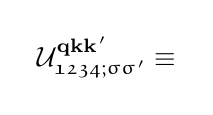
\begin{tikzpicture}[baseline=(current bounding box.center)]
	\node{$\mathcal{U}^{\textbf{qkk}'}_{\mathfrak{1234};\sigma\sigma'}\equiv$};
\end{tikzpicture}
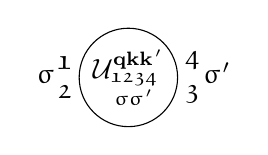
\begin{tikzpicture}[baseline=(current bounding box.center)]
	\coordinate (a) at (0,0);
	\coordinate (b) at (1.25,0);
	
	\node[above left=-0.1em of a] (n1) {$\mathfrak{1}$};
	\node[below left=-0.1em of a] (n2) {$\mathfrak{2}$};
	\node[below right=-0.1em of b] (n3) {$\mathfrak{3}$};
	\node[above right=-0.1em of b] (n4) {$\mathfrak{4}$};
	\node[left=0.2cm of a] (s1) {$\sigma$};
	\node (s2) at ($(b)+(0.5,0.05)$) {$\sigma'$};
	
	\node (centre) at ($(a)!0.5!(b)$) {$\mathcal{U}^{\textbf{qkk}'}_{\substack{\mathfrak{1234}\\\sigma\sigma'}}$};
	
	\draw (centre) circle (0.625);
\end{tikzpicture}
\begin{tikzpicture}[baseline=(current bounding box.center)]
	\node{$=$};
\end{tikzpicture}
\raisebox{1mm}{
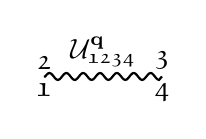
\begin{tikzpicture}[baseline=(current bounding box.center)]
	\begin{feynman}
		\vertex (a);
		\vertex[right=0.75cm of a] (b);
		\vertex[right=0.75cm of b] (c);
		
		\vertex[below=-0.1em of a] (n1) {$\mathfrak{1}$};
		\vertex[above=-0.1em of a] (n2) {$\mathfrak{2}$};
		\vertex[above=-0.1em of c] (n3) {$\mathfrak{3}$};
		\vertex[below=-0.1em of c] (n4) {$\mathfrak{4}$};	
		
		\vertex[above=0em of b] (u) {$\mathcal{U}^{\textbf{q}}_{\mathfrak{1234}}$};
		
		\diagram* {
			(a) -- [photon, thick] (c),		
		};
	\end{feynman}
\end{tikzpicture}}
\begin{tikzpicture}[baseline=(current bounding box.center)]
	\node{$-$};
\end{tikzpicture}
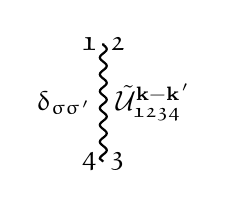
\begin{tikzpicture}[baseline=(current bounding box.center)]
	\begin{feynman}
		\vertex (a);
		\vertex[below=0.75cm of a] (b);
		\vertex[below=0.75cm of b] (c);
		
		\vertex[left=-0.1em of a] (n1) {$\mathfrak{1}$};
		\vertex[left=-0.1em of c] (n2) {$\mathfrak{4}$};
		\vertex[right=-0.1em of c] (n3) {$\mathfrak{3}$};
		\vertex[right=-0.1em of a] (n4) {$\mathfrak{2}$};
		
		\vertex[left=0.1em of b] (u) {$\delta_{\sigma\sigma'}$};
		\vertex[right=0.1em of b] (u) {$\tilde{\mathcal{U}}^{\textbf{k}-\textbf{k}'}_{\mathfrak{1234}}$};
		
		\diagram* {
			(a) -- [photon, thick] (c),		
		};
	\end{feynman}
\end{tikzpicture}

\end{document}